\documentclass[10pt]{article}

\usepackage[utf8x]{inputenc}
\usepackage[english]{babel}
\usepackage{amsfonts}
\usepackage{amsmath}
\usepackage{amssymb}
\usepackage{url}
\usepackage{bookmark}
\usepackage{hyperref}
\usepackage{fancyhdr} 
\usepackage{youngtab}
\usepackage[
    type={CC},
    modifier={by-nc-sa},
    version={4.0},
]{doclicense}

\pagestyle{fancy}
\fancyhf{}
\lfoot{\small \url{https://tingfengx.github.io/uoftnotes/}}
\lhead{\leftmark}
\rfoot{Page \thepage}

% customized commands
\newcommand{\settag}[1]{\renewcommand{\theenumi}{#1}}
\newcommand{\R}{\mathbb{R}}
\newcommand{\real}{\mathbb{R}}
\newcommand{\complex}{\mathbb{C}}
\newcommand{\field}{\mathbb{F}}
\newcommand{\double}[1]{\mathbb{#1}} % Set to behave like that on word
\newcommand{\qed}{\hfill $\mathcal{Q}.\mathcal{E}.\mathcal{D}.\dagger$}
\newcommand{\tbf}[1]{\textbf{#1}}
\newcommand{\tit}[1]{\textit{#1}}
\newcommand{\contradiction}{$\longrightarrow\!\longleftarrow$}
\newcommand{\overbar}[1]{\mkern 1.5mu\overline{\mkern-1.5mu#1\mkern-1.5mu}\mkern 1.5mu}
\newcommand{\proof}{\tit{\underline{Proof:}}} % This equivalent to the \begin{proof}\end{proof} block
\newcommand{\proofforward}{\tit{\underline{Proof($\implies$):}}}
\newcommand{\proofback}{\tit{\underline{Proof($\impliedby$):}}}
\newcommand{\proofsuperset}{\tit{\underline{Proof($\supseteq$):}}}
\newcommand{\proofsubset}{\tit{\underline{Proof($\subseteq$):}}}
\newcommand{\trans}[3]{$#1:#2\rightarrow{}#3$}
\newcommand{\map}[3]{\text{$\left[#1\right]_{#2}^{#3}$}}
\newcommand{\dime}[1]{\text{dim}(#1)}
\newcommand{\mat}[2]{M_{#1 \times #2}(\R)}
\newcommand{\aug}{\fboxsep=-\fboxrule\!\!\!\fbox{\strut}\!\!\!}
\newcommand{\basecase}{\textsc{\underline{Basis Case:}} }
\newcommand{\inductive}{\textsc{\underline{Inductive Step:}} }
\newcommand{\norm}[1]{\left\lVert#1\right\rVert}
% Call settag{\ldots} first to initialize, and then \para{} for a new paragraph
\newcommand{\va}{\mathbf{a}}
\newcommand{\vb}{\mathbf{b}}
\newcommand{\vv}{\mathbf{v}}
\newcommand{\vu}{\mathbf{u}}
\newcommand{\vw}{\mathbf{w}}
\newcommand{\vx}{\mathbf{x}}
\newcommand{\ve}{\mathbf{e}}
\newcommand{\vy}{\mathbf{y}}
\newcommand{\vz}{\mathbf{z}}
\newcommand{\vc}{\mathbf{c}}
\newcommand{\vm}{\mathbf{m}}
\newcommand{\vh}{\mathbf{h}}
\newcommand{\vzero}{\mathbf{0}}
% For convenience, I am setting both of these to refer to the same thing.
\newcommand{\ba}{\mathbf{a}}
\newcommand{\bb}{\mathbf{b}}
\newcommand{\bv}{\mathbf{v}}
\newcommand{\bu}{\mathbf{u}}
\newcommand{\bw}{\mathbf{w}}
\newcommand{\bx}{\mathbf{x}}
\newcommand{\be}{\mathbf{e}}
\newcommand{\by}{\mathbf{y}}
\newcommand{\bzero}{\mathbf{0}}
\newcommand{\boldf}{\mathbf{f}}
\newcommand{\bg}{\mathbf{g}}
\newcommand{\bm}{\mathbf{m}}
\newenvironment{rcases}
  {\left.\begin{aligned}}
  {\end{aligned}\right\rbrace}

\title{Miscellaneous notes in Algorithm Design, Analysis and Complexity}
\author{\ccLogo \,\,Tingfeng Xia}
\date{Fall 2019, modified on \today}

\begin{document}
\maketitle
\doclicenseThis
\tableofcontents
\newpage

\section{6.046J Linear Programming: LP, Reductions, Simplex}
\subsection{Example: Politics, example of optimization}
\begin{itemize}
    \item Goal: You want to buy elections and you want to minimize the total amount of money spent. 
    \item How to campaign to win an election? Manager estimates votes obtianed per dollar spent.
\end{itemize}
\begin{center}
    \begin{tabular}{|c|c||c|c|c|}
        \hline
         & Policy & Urban & Suburban & Rural \\
        \hline
        \hline
        $x_1$ & Build Roads & -2 & 5 & 3 \\
        \hline
        $x_2$ & Gun Control & 8 & 2 & -5 \\
        \hline
        $x_3$ & Farm Subsidies & 0 & 0 & 10 \\
        \hline
        $x_4$ & Gasoline Tax & 10 & 0 & 2 \\
        \hline
    \end{tabular}
\end{center}
\begin{itemize}
    \item Want a mojority for each demographic. 
\end{itemize}
\begin{center}
    \begin{tabular}{|c||c|c|c|}
        \hline
        Polulation & 100,000 & 200,000 & 50,000 \\
        \hline
        Majority & 50,000 & 100,000 & 25,000 \\
        \hline
    \end{tabular}
\end{center}
\begin{itemize}
    \item Want to win by spending the minimum amount of money.
    \item Algebraic Setup: Let $x_1,x_2,x_3,x_4$ denote the dollar spent per issue. 
        $$
        \begin{cases}
            \text{minimize} &x_1 + x_2 + x_3 + x_4 \\
            \text{subject to} &(1)~~ -2x_1 + 8x_2 + 0x_3 + 10x_4 \geq 50000 \\
            &(2)~~5x_1 +2x_2 +0x_3 +0x_4 \geq 100000 \\
            &(3)~~ 3x_1 - 5x_2 + 10x_3 - 2x_4 \geq 25000 \\
            &(4)~~ x_1,x_2,x_3,x_4 \in \real^{\geq 0}
        \end{cases}
        $$
    Notice that constraint (4) above denotes there is no negative advertisation. 
    \item The optimal solution is 
        $$
        \begin{cases}
            x_1 = 2050000/111 \\
            x_2 = 425000/111 \\
            x_3 = 0 \\
            x_4 = 625000/111
        \end{cases}
        $$
        and the objective optimized has value $\frac{3100000}{111}$
\end{itemize}

\subsection{Standard From for LP}
\begin{itemize}
    \item Minimize or Maximize\footnote{In the standard form, we consider the maximization problem} linear objective function, subject to linear ineqalities or equations
    \item Variables $\bx = [x_1,x_2,\dots,x_n]^T$, and the objective function is $\mathbf{c} \cdot \bx = c_1x_1 + \dots + c_nx_n$ and the ineqalities $\mathbf{A}\cdot \bx \leq \mathbf{b}$\footnote{In general, this could have been $\leq, \geq, =$ but for the standard form, we consider $\leq$} and $\bx \geq \mathbf{0}$\footnote{Meaning that each of the slots in the vector should be greater than zero.}
\end{itemize}

\subsection{Certificate of Optimality}
\paragraph{Is there a short certificate?}\footnote{For the problem of Politics described above, notice that this is not a general certificate, it only works in this specific case.}  
Consider $$25/222 (1) + 46/222 (2) + 14/222 (3)$$, where we can plug in the equations and simplify to $$x_1 + x_2 + 140/222  x_3 + x_4 \geq 3100000/111$$
But notice that $$3100000/111 \leq x_1 + x_2 + 140/222  x_3 + x_4 \leq x_1 + x_2 + x_3 + x_4$$ so the solution must be optimal!

\subsection{LP Duality} 
\paragraph{What is this?} This is essentially saying that what we did above was no coincidence, and we can always to this for a linear program. 

\paragraph{Theorem} For all standard form of LP (called a primal form) there exists a dual form that is equivalent to the primal. Specifically
\begin{equation*}
    \begin{rcases}
        \text{maximize~~} &\mathbf{c}\cdot \mathbf{x}\\
        \text{subject to~~} &A\bx \leq \mathbf{b} \\
                        &\bx \geq \mathbf{0}
    \end{rcases}
    \quad \equiv \quad 
    \begin{cases}
        \text{minimize} &\mathbf{b}\cdot \by \\
        \text{subject to} &A^T \by \geq \mathbf{c} \\
                        &\mathbf{y} \geq \mathbf{0}
    \end{cases}
\end{equation*}

\subsection{Converting to Standard Form}
\subsubsection{Case 1: Minimize Goal} Suppose that I want to minimize $-2x_1 + 3x_2$, then I can just convert the problem into maximizing the negative of the equation. This case should be easy.
\subsubsection{Case 2: Missing Non-negative Constraint} Suppose $x_j$ doesn't have a non-negative constraint. In this case, we will replace $x_j$ with $x_j' - x_j''$ such that $x_j' \geq 0\land x_j'' \geq 0$. 
\subsubsection{Case 3: Equlity Constraint} Suppose the constriant was $x_1 + x_2 = 7$, then we can break it into $x_1 + x_2 \leq y \land -x_1 - x_2 \leq -7$.\footnote{Notice that we did this in this specific way becasue we want to have this in out standard form where the constraint was a $\leq$. The second constraint here, if we multiply it by $-1$ on both sides, is equivalent to saying $x_1+x_2 \geq 7$}
\subsubsection{Case 4: GEQ Constraint} We have done this above, translate this into a less than or equal tot problem by multiplying $(-1)$ on both sides (which will flip the ineqality sign).

\subsection{Max-Flow using LP}
Consider some network $N:= G = (V,E)$, and denote the flow in the network to be $f$. the function $c(\cdot)$ returns the capacity for an edge. The problems then breaks into
$$
\begin{cases}
    \text{maximize} &\sum_{v\in V} f(s,v) = |f| \\
    \text{subject to} &f(u,v) = -f(v,u)~~\forall u, v \in V \\
    &\sum_{v\in V}f(u,v) = 0 ~~\forall u \in V\setminus\{s, t\} \\
    &f(u,v) \leq c(u,v) ~~\forall u,v \in V
\end{cases}
$$
where we notice that the above problem is entirely linear and thus could be solved using a linear programming algorithm.

\paragraph{Time Complexity} This generalization uisng LP is much slower than the network flow algorithms (Ford-Fulkerson, Edmonds-Karp, et cetra) in \textbf{single commodity network flow}. 

\paragraph{Multi-Commodity Flow} Consider the case where there are two commodities flowing in the network ($f_1, c_1, f_2, c_2$). In the case where $c_1$ is independent from $c_2$, it is not very interesting, we can just run the network flow algorithm twice to find two maximizers seperately. In the case where there is a single capacity constraint $c$\footnote{A toy example to give would be given a certain road where some cars are running on the road and the raod have a total capacity for all types of cars combined}, the problem ceases to be a simple network flow problem. However, it is still easy to come up with a LP formulation that describes the maximization. 

\subsection{Shortest Path using LP}
\begin{itemize}
    \item $d[v]$ represents the shortest path from the source to $v$\footnote{It might be helpful to recall that in the Dijkstra's Algorithm $d[v]\gets \infty$ initially and then it was decremented through out the algorithm until the minimum was reached.} 
    \item $w(u,v)$ means the single edge $(u,v)$'s weight
    \item The shortest path to some vertex $v$ which is a descendent of $u$ is at least shorter than or equal to the existing path that goes from source to $u$ plus the edge $(u,v)$
    \item The shortest path from source to source is zero
    \item Recall the $\triangle$-ineqality here
\end{itemize}
This yields the formulation
\begin{equation*}
    \begin{cases}
        \text{maximize} &d[v] \\
        \text{subject to} &d[v] - d[u] \leq w(u,v)~~\forall (u,v) \in E \\
        &d[s] = 0 \\
        &d[v] - d[u_1] \leq w(u_1, v) \\
        &d[v] - d[u_2] \leq w(u_2, v) \\
        &d[v] = \min(\dots,\dots)
    \end{cases}
\end{equation*}
Notice that although we are trying to minimize the distance from source to the node $v$, we have to put this as a maximization problem because otherwise the trivial solution of $0$ will work! Our formulation didn't capture the insight ``We DO want a path''.

\paragraph{Key Insight of MAX} The above formulation already captured the minimization problem with the min in the last constraint and hence we want to push up as hard as we can in finding a solution. (We are ANDing together all the constraints and have chosen the one that is the smallest)

\subsection{Simplex Algorithm}

\subsubsection{Work Flow}
\begin{enumerate}
    \item Represent LP in slack form
    \item Convert one slack form into an equivalent whose objective value has not decreased and has likely increased (no gurantee of increase)
    \item Keep going until the optimal solution becomes obvious
\end{enumerate}

\subsubsection{Time Complexity} This is, unfortunately, an exponential iterative algorithm. Denote the number of constraints using $m$ and $n$ as the number of variables then the algorithm has worst case time complexity 
\begin{equation*}
    T(m,n) \in \mathcal{O}\left(\binom{m+n}{n}\right)
\end{equation*}

\subsubsection{Procedure Example}
Consider the problem
$$
\begin{cases}
    \text{maximize} & 3x_1 + x_2 + x_3 \\
    \text{subject to} &x_1 + x_2 + x_3 \leq 30 \\
    &2x_1 + 2x_2 + 5x_3 \leq 24 \\
    &4x_1 + x_2 + 2x_3 \leq 36 \\
    &x_1,x_2,x_3\geq 0
\end{cases}
$$

\paragraph{The Slack From}\footnote{Here the word `slack' means how much room is still left} The original variables ($x_1, x_2, x_3$ here) will be called non-basic variables and we will here introduce three \textit{basic} variables\footnote{This amount will be equal to the number of constraints that the original problem have} $x_4, x_5$ and $x_6$. The original problem will then be
\begin{equation*}
    \begin{cases}
        z = 3x_1 + x_2 +x_3 \\
        \begin{rcases}
            x_4 &= 30 - x_1 - x_2 - x_3 \\
            x_5 &= 24 - 2x_1 - 2x_2 - 5x_3 \\
            x_6 &= 36 - 4x_1 - x_2 - 2x_3
        \end{rcases}
        (I)
    \end{cases}
\end{equation*}
It is worth mentioning that now the non-negativity constriant becomes $\real^6 \ni \bx \geq \vzero$, we have ``added''\footnote{This was quoted because we didn't actually introduce any new constraints! In fact, they are pair-wise equivalent to the original ones.} three more new variables that are also non-negative.

\paragraph{Basic Solution} Set all the non-basic variables to zero, and then compute the values of the basic variables. The objective function will be $z = 3(0) + 1(0) + 1(0) = 0$. This is a trivial starting point and we can think of this solution as $\real^6 \ni \bx = (0,0,0,30, 24, 30)$

\paragraph{Pivoting} 
\begin{itemize}
    \item Select a non-basic variable $x_e$ whose coefficient in the objective function is positive
    \item Increment the value of $x_e$ as much as possible without violating any of the constraints. 
    \item Varaible $x_e$ becomes basic, some other variable becomes non-basic. (Value of the other basic variable and the objective function may change.) 
\end{itemize}

\paragraph{Running the Procedure}
\begin{itemize}
    \item Suppose we selected the non-basic variable $x_e = x_1$ and we want to increase the value of $x_1$. 
    \item The third constraint is the tighest one in (I). Rearrange the terms we have 
        \begin{equation}
            x_1 = 9 - x_2/4 - x_3/2 - x_6/4
        \end{equation}
    \item Then we will rewrite the other equations with $x_6$ on the RHS. i.e. replace all occurences of $x_1$ with (1) above. \textbf{Important:} What has happened is that $x_1$ and $x_6$ has exchanged their roles. $x_1$ was non-basic and will now become basic and is the reverse for $x_6$. The following is the re-written result:
        \begin{equation*}
            \begin{cases}
                \begin{rcases}
                z &= 27 + x_2/4 + x_3/2 - 3x_6 /4 \\
                x_1 &= 9 - x_2/4 - x_3/2 - x_6/4 \\
                x_4 &= 21 - 3x_2/4 - 5x_3/2 +  x_6/4 \\
                x_5 &= 6 - 3x_2/2 - 4x_3 + x_1/2 
                \end{rcases}
                (II)
            \end{cases}
        \end{equation*}
    \textbf{Point of the above operation:} Recall the original basic solution was $(0,0,0,30,24,36)$, which certainly satisfies (II) above and have objective value
        \begin{equation*}
            27 + \frac{1}{4}(0) + \frac{1}{2}(0) - \frac{3}{4}(36) = 0
        \end{equation*}
    For the basic solution for (II), we set the non-basic values to zero which will yield the solution $(9,0,0,21,6,0)$\footnote{The solution was computed by setting variables on the RHS of the equations (which are the non-basic vars now) to zero in (II)}. The objective value is now $3x_1+x_2 + x_3 = 9 \times 3 = 27$.\footnote{The original objective function was used here}
    \item Repeat the above procesure. In this case, 2 more iterations is required. We will know it is the time to stop when the objective function is some constant followed by negative copies of non-basic variables (which are non-negative) in which case the objective fucntion cannot be increased anymore. We call this the convergence of the Simplex Algorithm.
\end{itemize}
  
\section{6.006 Computational Complexity}
\subsection{Complexity Classes}
\begin{itemize}
    \item \textbf{P} Set of all problems that can be solved in less than or equal to polynomial time.
    \item \textbf{NP} Decision problems that can be solved in polynomial time via a lucky algorithm.
    \item \textbf{NP-Hard} As hard as every problem in NP.
    \item \textbf{NP-Complete} NP $\cap$ NP-Hard.
    \item \textbf{EXP} Set of all problems that can be solved in less than or equal to exponential time.
    \item \textbf{R} Set of all problems that can be computed/solved in finite time
\end{itemize}

\subsubsection{Theorem: Alomost All Decision Problems are not in R}
This might be counter-intuitive but is mathematically valid. We are here limiting our scope to decision problems only, which is defined as `problems that outputs yes/no (some binary outcome)'. We will now prove this result, \textit{Proof:}
\begin{itemize}
    \item First, note that a program, what we write on a computer, is just a bianry string in some sense. But if it could be represented in a binary number (which might be a very big one), it is just a natural number in base 2. This is our space of programs.
    \item Next, a decision problem is a funtion that is $f: \text{input} \rightarrow \{\text{YES}, \text{NO}\}$. But for sure the input for a program is some string which could be converted into binary which is again some natural number. Hence, our $f$ is one such that $f:\mathbb{N} \rightarrow \{\text{YES}, \text{NO}\}$. 
    \item Above, we have argued that a program is a finite string of bits, while a decision problem is a infinite string of bits\footnote{For different inputs, the output may or may not be the same but importantly is never stops, i.e. there always exists the next problem.}.
    \item Hence, decision problems $\in \real$ while programs is $\in \mathbb{N}$. But $|\mathbb{R}| \gg |\mathbb{N}|$! So there is not enough program to solve all the decision problems. 
\end{itemize}
\hfill $\blacksquare$

\subsection{The Big Conjecture}
\begin{equation*}
    P\neq NP \approx \text{``You can't engineer luck''}
\end{equation*}

\subsection{Reductions}
\paragraph{The idea} is to convert some problem A into a problem B. When we can reduce A to B, we say B is as hard as A. 
\paragraph{Example I} To solve unweighted shortest paths, we can use a BFS. But for sure we can also solve this using Dijkstra by setting all the weights to one. This would be an example of a reduction. 
\paragraph{Example II} Suppose we want to, again, solve the shortest path (weighted) problem but we are only given the tool of `min-product path'\footnote{That is, minimize the product of the weights along the path}. You can do this by taking logs, after which products become sum!

\section{6.046J Complexity: P, NP, NP-Completeness, Reductions}

\subsection{Definitions}
\begin{itemize}
    \item \textbf{NP} Given any instance $I$ of problem $P$ and witness $W$, if there exists a verifier $V$ so that given the ordered pair $(I, W)$ as input, $V$ returns ``yes'' in polynomial time if the witness proves that the answer is ``yes'' and ``no'' in polynomial time otherwise, then $P$ is in NP. \textbf{Important:} Notice that to show that a problem is in NP, we have to consider all possible certificates ($\forall$ quantified) and for each certificate there should exist some verfier (which could certainly be different each time). 
    \item \textbf{NP-Completeness} A problem X is NP-Complete if X$\in$NP and X$\in $NP-Hard
    \item \textbf{NP-Hard} X is NP-Hard if every problem Y$\in$NP reduces to X.
    \item \textbf{Redution} from problem A to a problem B = poly-time algorithm converting A inputs to some equivalent B inputs.\footnote{Two important observations here: 1. if B in P then A in P; 2. if B in NP then A in NP}
\end{itemize}

\subsection{Class Relationships}
\begin{center}
    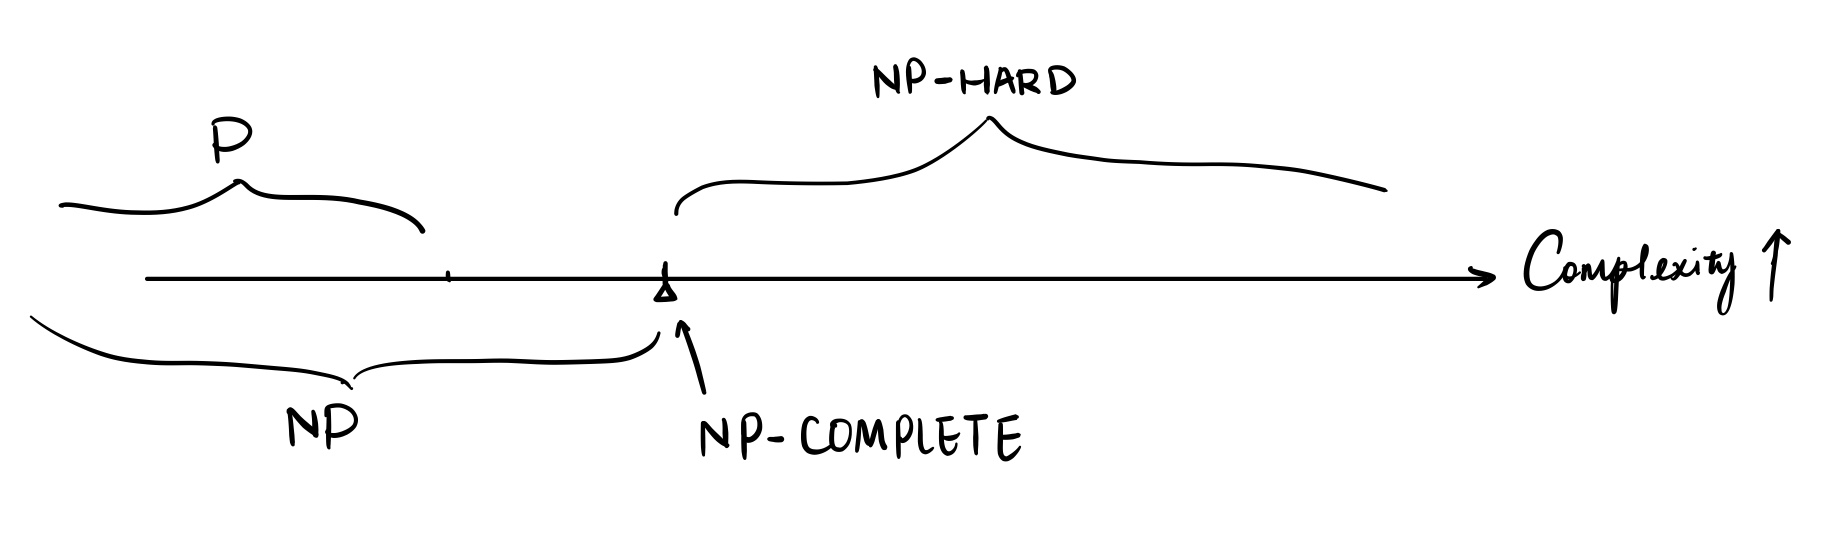
\includegraphics[scale=0.16]{img/compare_complexities.jpg}
\end{center}

\subsection{Proving NP-Completeness}
From a algorithm perspective, the question is `How to prove X is NP-Complete?'
\begin{enumerate}
    \item Show that X in NP. (Give a non-detrministeic algorithm OR give a certificate and verify.)
    \item Reduce from some known NP-Complete problem Y to your problem X. \textbf{Important:} Always reduce from the thing that you know is hard to the thing that you want to show is hard. This direction matters. 
\end{enumerate}

\subsection{3 SAT} Given a boolean formula, which is an AND of triplet ORs. A clause is one of the triplet ORs and a literal is one element in a triplet OR. The question is does there exist a assignment of variables such that the final result (the entire boolean formula) evaluates to true. 
\paragraph{Intuition behind the Proof of NP-Completeness of 3 SAT}
\begin{itemize}
    \item Software $\approx$ Hardware, you can build a circuit for a software/algorithm using logic gates
    \item If I have a circuit, than I can convert that into a boolean formula.
    \item (Fun Fact; Less obvious) If I have formula, then I can convert it into the form 3 SAT problem requires. 
    \item Then the `witness/oracle' is described by the literals in the formula
    \item Then deciding whether there's some way to set the literals to make the formula true is the same thing as saying `Is there some certificate where the verifier says yes', which is the same thing as saying that the problem has answer yes.
\end{itemize}

\subsection{3-Dimensional Matching (3DM)}
\paragraph{Problem Statement} You are given disjoint sets $X, Y$ and $Z$, each of size $n$. You are also given triples $T\subseteq X\times Y \times Z$. The goal is to choose subset $S\subseteq T$ such that every element $\in X \cup Y \cup Z$ is in exactly one $s\in S$. 

\paragraph{Reducing From 3 SAT} 
We will need the following three gadgets, namely the variable gadget, the garbage collection gadget, and the clause gadget. 
\begin{center}
    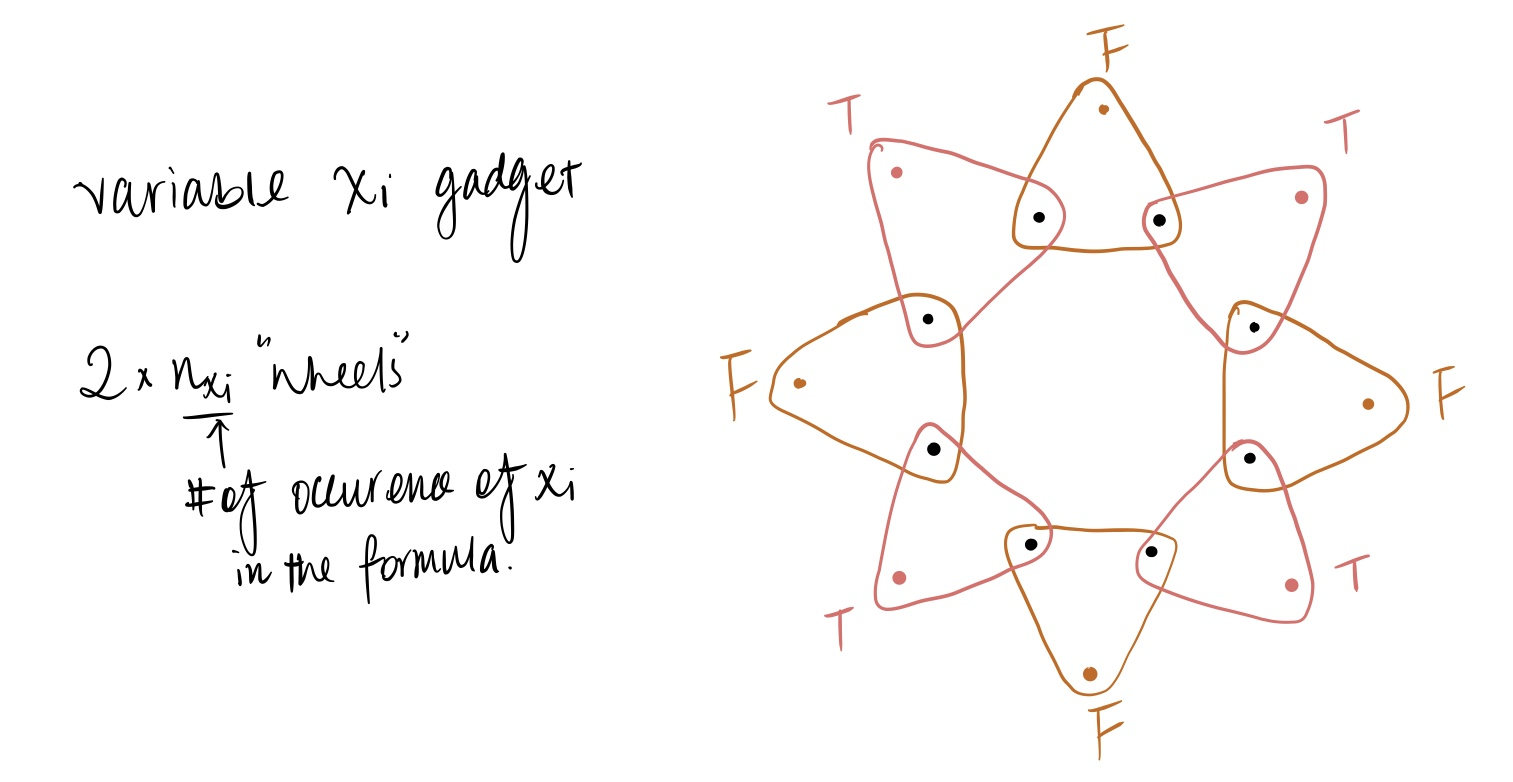
\includegraphics[scale=0.22]{img/3dm_variable.jpg}
    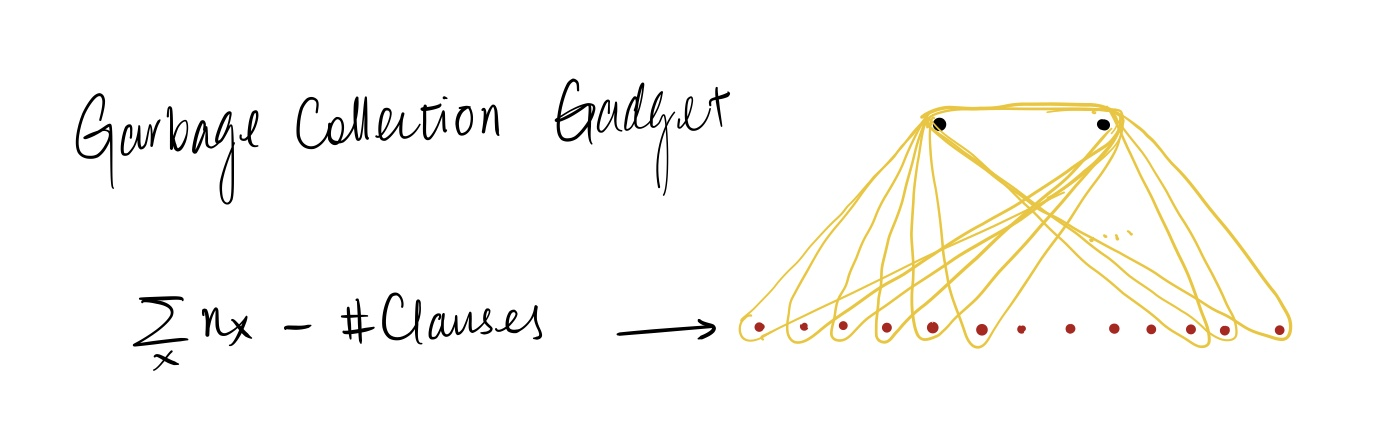
\includegraphics[scale=0.22]{img/3dm_garbage.jpg}
    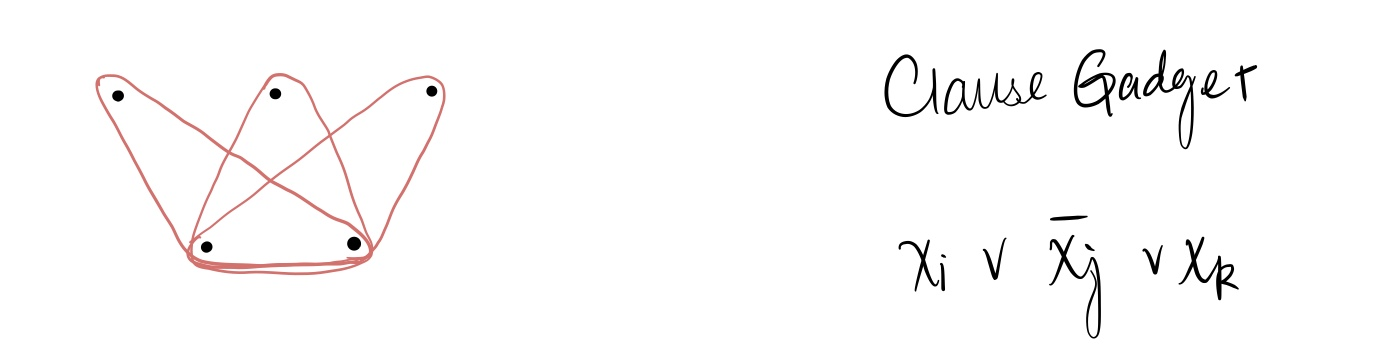
\includegraphics[scale=0.22]{img/3dm_clause.jpg}
\end{center}
\begin{itemize}
    \item In the variable gadget, the dots on the inner circle exists in only that gadget, and there is a variable gadget for each and every variable.
    \item The reason that we have $2n_{x_i}$ sized\footnote{Notice that here $n_{x_i}$ counts all occurences of the variable $x_i$, including the $\overbar{x_i}$'s} variable gadgets is that here in the wheel we are only allowed to choose all the T's or all the F's but not mixed. This way, we have twice the number of needed variable connectors and then we choose half of them which is exactly what we need for the gadget to work. 
    \item The clause gadget has the two dots on the lower level local and the top three are connected to the outer T/F dots on the variable gadgets. Notice that we are only allowed to choose one of the three triangles in the gadget drawn. Importantly, the one choice gurantees the bottom two nodes are chosen, meaning the clause is satisfied. 
    \item Doing the above is not enough since then not all T/F nodes\footnote{That is, all the top three nodes in all the clause gadgets and all the nodes in the outer ring in the variable gadgets} will be used which is problematic. To solve this, we add a garbage collection gadget.
    \item The Garbage Collection Gadget has all the T/F nodes on its lower row, and the gadget itself is repeated $\sum_x n_x - \#Clause$ times. This will help to connect all the unconnected nodes left from the previous steps.  
\end{itemize}

\subsection{Subset Sum}
\paragraph{Problem Statement} Given $n$ integers $A = \{a_1, ..., a_n\}$ and target sum $t$. Does there exist a subset sum $S\subseteq A$ such that $\sum S = \sum_{a_i \in S} a_i = t$, i.e. adds up to a given sum.
\paragraph{Reducing From 3DM}
\begin{itemize}
    \item View numbers in base $b = 1 + \max_i n_{n_i}$, a large enough base. The max part is the total number of colliding ones and we are setting our base to be one larger than that so that there will never be carries. 
    \item Triple $(x_i, x_j, x_k)$ will be converted into \texttt{0000100001001000$_b$} where the $1$'s are at the $i,j,k$-th position in the number.
    \item The goal is to add up to some number $1111111111 = \sum_{i'} b^{i}$
\end{itemize}
\textbf{How does this reduction work?} Notice that my goal now in base $b$ is a bunch of ones, and I am trying to add up to this number from numbers in base $b$ composed of three 1's and 0's on the rest positions. So, I need to gurantee that there is no collision meaning no two occurences of 1 on the same position will be accepted. Then, the problem is essentially choosing non-overlapping subsets that can add up to the target number which is exactly what 3DM solves. \qed

\paragraph{Weakly NP-Hardness} The numbers in the above reduction are giant. The number of digits in the target number in base $b$ have order $\mathcal{O}(n)$ digits. But, the actual values of the numbers are exponential, and this is not allowed in a Strong NP-Hardness setting. 

\subsection{Partition}
\paragraph{Problem Statement} Given $A = \{a_1,...,a_n\}$ integers, is there a subset $S\subseteq A$ such that  $\sum S = \sum S\setminus A$, i.e. the set is partitioned into two parts that adds up to the same numeber.
\paragraph{Reducing From Subset Sum}
\begin{itemize}
    \item Let $t$ denote the arbitrary target of my Subset Sum instance
    \item Let $\sigma = \sum A$
    \item Add $a_{n+1} = \sigma + t$ and $a_{n+2} = 2\sigma - t$
    \item After adding the two terms described above, we first note that they can't be on the same side in the partition, because if they do then one side would have sum at least $\sigma + t + 2\sigma - t = 3 \sigma$ which is way larger than $\sigma$, the total sum of all numbers. 
    \item Now we know that these two numbers have to be on two sides of the partition, we notice that if we add $\sigma - t$ to the side that has $a_{n+1} = \sigma + t$ and add $t$ to the other side, then both sides will have sum $2\sigma$, which is what we want. 
    \item Starring at the above step, we notice that $\sigma - t + t = \sigma$ is the total sum of elements that we want to add to two sides of the partition, which is exactly equal to the total sum of all the original $n$ elements! 
    \item Then, if this partition problem could be solved, my subset sum of arbitrary target $t$ can be solved and this shows Subset Sum could be $p$-reduced to Partition. 
\end{itemize}


\subsection{My Thorughts}
\paragraph{P-Reducibility} $A \leq_p B$ means $A$ is $p$-reducible to $B$. To show this is true, we have to take an arbitrary input of $A$, and find a polynomial time conversion such that this input is now a appropriate input for $B$. Then we will let $B$ solve this problem for us, and we will need a polynomial time conversion back from $B$'s solution to the required $A$'s. 

\paragraph{Mario Reduced From 3 SAT} We tried to show that 3 SAT $\leq_p$ Mario, i.e. 3 SAT is $p$-reducible to Mario. Given any instance of 3 SAT problem\footnote{By instance of a problem, we mean that the input of the problem, which will be translated to the input of some other problem and from where the solution yielded will be converted back and thus act as the solution to `the instance of a problem'.}, we can build a respective level for Mario and whether Mario dies or not will tell us if 3 SAT should return YES or NO. 

\paragraph{Partition Reduced From Subset Sum} (Subset Sum $\leq_p$ Partition) Given a Subset Sum problem, we add two elements into the set and give this as the input to the Partition solver. If the partition solver was able to return a YES solution, then we know that the elements in the partitions which 
contains the $2\sigma - t$ element (exclude the $2\sigma - t$ element) has subset sum equal to $t$ which means the Subset Sum could be solved by using Partition as a black box. 

















\end{document}
